\chapter{\textit{Commit History} dari Kontributor}

Buku ini merupakan hasil karya bersama dari beberapa penulis. Peran masing-masing penulis bisa dilihat pada bagian Gambar~\ref{fig:commitHistory}. Ada 2 nama ``Bambang Purnomosidi D. P.'' disitu. Keduanya adalah orang yang sama, tetapi pada saat \textit{commit}, ada satu yang dilakukan di komputer lain dengan konfigurasi git yang berbeda (pada file gitconfig), khususnya di alamat email sehingga dikenali sebagai kontributor lain oleh Github.

  \begin{figure}
    \begin{center}
      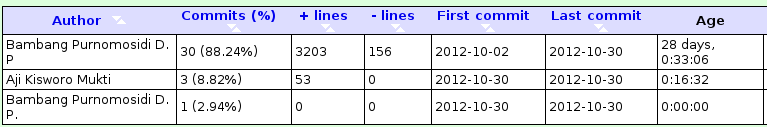
\includegraphics[scale=0.5]{images/appendixCommitHistory.png}
    \end{center}
    \caption{\textit{Commit history} dari penulisan buku}
    \label{fig:commitHistory}
  \end{figure}



